%%\documentclass[12pt]{article}
\documentclass[12pt]{elsarticle}
\usepackage{graphicx}
\usepackage{subfig}
\usepackage{amssymb,hyperref,rotating}
%\usepackage{draftwatermark}
%\SetWatermarkScale{2.0}
%\usepackage{dcolumn}
%\usepackage{bm}
%\documentstyle{psfig,epsf}{article}
%\usepackage{psfig,wrapfig,floatfig,float}
%\topmargin 0.5cm
%\addtolength{\evensidemargin}{-1.5cm}
%\addtolength{\oddsidemargin}{-1.5cm}
%\addtolength{\textwidth}{2.54cm}
%\addtolength{\topmargin}{-1.5cm}
%\addtolength{\textheight}{2.54cm}

\topmargin=-0.25in
\textwidth=6.25in
\textheight=8.25in
%\textheight=9.25in
\oddsidemargin=0.125in
\evensidemargin=0.125in

%\addtolength{\textwidth}\larsoft{1.2in}
%\addtolength{\topmargin}{-.7in}
%\addtolength{\leftmargin}{-1.1in}
%\addtolength{\footskip}{-1.5cm}
%%\setlength{\textheight}{9.25in}
%\setlength{\textheight}{9.3in}
%%\setlength{\parindent}{1em}
%\setlength{\parskip}{1ex}
%%\pagestyle{headings}
%\setlength{\oddsidemargin}{0.in}
%\setlength{\evensidemargin}{0.in}
\newcommand{\larsoft}{LArSoft }
\thispagestyle{empty}

\pagestyle{myheadings}
\begin{document}
\title{The Liquid Argon Offline Software Package: \larsoft} 
\author{Jonathan Asaadi}
\address{}
\ead{jaasaadi@syr.edu}
\author{Bruce Baller}
\address{}
\ead{baller@fnal.gov}
\author{Ben Carls}
\address{}
\ead{bcarls@fnal.gov}
\author{Eric Church}
\address{Physics Department, Yale University, New Haven, CT, USA, 12345-1234}
\ead{echurch@fnal.gov}
\author{Bonnie Fleming}
\address{Physics Department, Yale University, New Haven, CT, USA, 12345-1234}
\ead{bonnie.fleming@yale.edu}
\author{Herb Greenlee}
\address{Fermi National Accelerator Lab, Batavia, IL, USA, 60510-5011}
\ead{greenlee@fnal.gov}
\author{Ben Jones}
\address{Massachusetts Institute of Technology, 77 Massachusetts Ave, Cambridge, MA 02139}
\ead{bjpjones@mit.edu}
\author{Thomas R. Junk}
\address{Fermi National Accelerator Lab, Batavia, IL, USA, 60510-5011}
\ead{trj@fnal.gov}
\author{Wes Ketchum}
\address{}
\ead{wketchum@lanl.gov}
\author{Jim B. Kowalkowski}
\address{Fermi National Accelerator Lab, Batavia, IL, USA, 60510-5011}
\ead{jbk@fnal.gov}
\author{David McKee}
\address{}
\ead{mckee-d@mssu.edu}
\author{Tia Miceli}
\address{Fermi National Accelerator Lab, Batavia, IL, USA, 60510-5011}
\ead{miceli@fnal.gov}
\author{Gianluca Petrillo}
\address{Fermi National Accelerator Lab, Batavia, IL, USA, 60510-5011}
\ead{petrillo@fnal.gov}
\author{Brian Rebel}
\address{Fermi National Accelerator Lab, Batavia, IL, USA, 60510-5011}
\ead{brebel@fnal.gov}
\author{William Seligman}
\address{Columbia University Nevis Laboratories, PO Box 137, Irvington, NY, USA, 10533}
\ead{seligman@nevis.columbia.edu}
\author{Erica Snider}
\address{Fermi National Accelerator Lab, Batavia, IL, USA, 60510-5011}
\ead{rs@fnal.gov}
\author{Mitchell Paul Soderberg}
\address{Fermi National Accelerator Lab, Batavia, IL, USA, 60510-5011}
\ead{soderber@fnal.gov}

\author{Andrzej Szelc}
\address{}
\ead{andrzej.szelc@yale.edu}

\author{Kazuhiro Terao}
\address{}
\ead{kazuhiro@nevis.columbia.edu}
\author{Matthew Toups}
\address{}
\ead{mtoups@mit.edu}
\author{Tingjun Yang}
\address{Fermi National Accelerator Lab, Batavia, IL, USA, 60510-5011}
\ead{tjyang@fnal.gov}
%%\hspace{2cm}                         
\begin{abstract}
A common software package for the simulation, reconstruction, and analysis of Liquid Argon TPC (LArTPC) detectors is being developed as a collaboration across multiple experiments at Fermilab, with the core framework supported by Laboratory staff. The architecture of the software and collaboration that provides the value delivered by the common package are described, along with the various components explaining the development and integration model for the common and experiment specific aspects including the core framework, detector geometry, electronics response, package configuration, and algorithms.

\end{abstract}
\tableofcontents

%%\large
%%%
%%%\clearpage
\maketitle
\hyphenation{Particle-List-Action}
\hyphenation{created responses assumed respon-sible language}
\section{Introduction}
\subsection{What is \larsoft}
\larsoft is a software package for the simulation, reconstruction, and analysis of all planned and running liquid argon experiments at Fermilab. Any Liquid Argon Time Projection Chamber (LArTPC) experiment can make use of \larsoft algorithms as long as the experiment supplies a properly formatted description of its detector geometry and electronics. 

\larsoft  benefits from the experience of multiple experiments.  Each LArTPC provides essentially the same basic information after accounting for small detector differences.  Thus, algorithms developed for one experiment can be directly used by another, as long as the differences in geometry are properly accounted for in the algorithms.  

A liquid argon detector and a sophisticated software toolkit can analyze event topologies typical of neutrino interactions that are difficult to parse and make sense of in traditional legacy technologies. Figure~(ADD bubble chamber and Liquid Argon results picture)
Liquid argon detectors see every nuance of the event. \larsoft applies reconstruction algorithms to identify clusters of energy deposit, tracks, particle showers, and interaction vertices.

\subsection{Who Uses \larsoft}
\larsoft is the product of the collaboration between the following experiments and Fermilab.
\begin{enumerate}
\item ArgoNeuT
\item LongBo
\item LArIAT
\item MicroBooNE
\item LBNE
\item LAr1-ND
\end{enumerate}

\hspace*{2cm}
\begin{figure}[h]
\centering
%\caption{\subfloat[]{\includegraphics[width=3.0in]{picture of bubble chamber}}%
%\caption{\subfloat[]{\includegraphics[width=3.0in]{picture of liquid argon}}%
\label{bubble}
\end{figure}

\section{Framework and Tools}
\subsection{ART}
The foundation of \larsoft is the ART event processing framework which coordinates event processing via configurable, pluggable modules that add data to, and retrieve data from, events.~\cite{art-ref}  An event is one unit of data. It may represent an interaction or any period of collected data.

ART provides many of the services necessary to operate in a production environment, including tools for compiling, installing, packaging, and deploying the system.  ART is developed and supported by the Fermilab Scientific Computing Division (SCD) and is used by experiments within the neutrino, astrophysics, and muon programs, including NOvA, Muon G-2, Mu2e, and DarkSide-50, and alongside \larsoft for MicroBooNE, ArgoNeuT, and Lariat.

\subsection{External Packages}
\subsubsection{Event Generation}
\larsoft makes use of the NuSoft packages that provide a common interface to event generators, Geant4 and event display libraries developed for use by all neutrino experiments. The packages used include: EventDisplayBase, EventGeneratorBase, G4Base, MagneticField, NuReweight and SimulationBase.

There are several different ways to create events for \larsoft:
\begin{enumerate}
\item{CRY - a third-party package to simulate cosmic rays~\cite{cry}}
\item{External neutrino interaction generators used to produce neutrinos in the Monte Carlo simulation. There are several generators which can supply input to \larsoft:}
\begin{enumerate}
\item{GENIE~\cite{genie} - the standard neutrino event generator in \larsoft}
\item{NuWro~\cite{nuwro} - a neutrino event generator with potentially improved spectral functions for liquid argon}
\item{GIBUU~\cite{gibuu} - a theory-code framework that was mainly developed for different classes of reactions other than neutrinos}
\item{NUANCE~\cite{nuance} - an older neutrino event generator used in MiniBooNE; it is available to compare the results of MiniBooNE and MicroBooNE simulations}
\end{enumerate}
\item{Single - creation of single participle spill or multiple particles with the initial position, momenta, and the spread of momenta and starting positions specified in the job file.}
\item{LightSource - simulation of placing an extended, isotropic light source within the TPC volume to generate a stream of photons.}
\item{TextFileGen - accepts a text file of HepMC~\cite{hepmc} event records.}
\end{enumerate}

\subsubsection{Detector Simulation}
NEED WORDS

\subsection{Geometry Description Requirements}
\label{sec-geom-desc}
\larsoft uses the Geometry Description Markup Language (GDML) which is an application-independent geometry description format based on Extensible Markup Language (XML.) 
The Geometry package contains a general interface into the detector descriptions of the different experiments so other packages do not depend on the detector. 

\begin{figure}[h]
\center
\caption{\larsoft requires a descending volume hierarchy of volWorld, volDetEnclosure, volCryostat, volTPC, volTPCPlane, volTPCWire to search for each of these specific volumes. There can be, and probably should be, multiple TPCPlanes and TPCWires.}
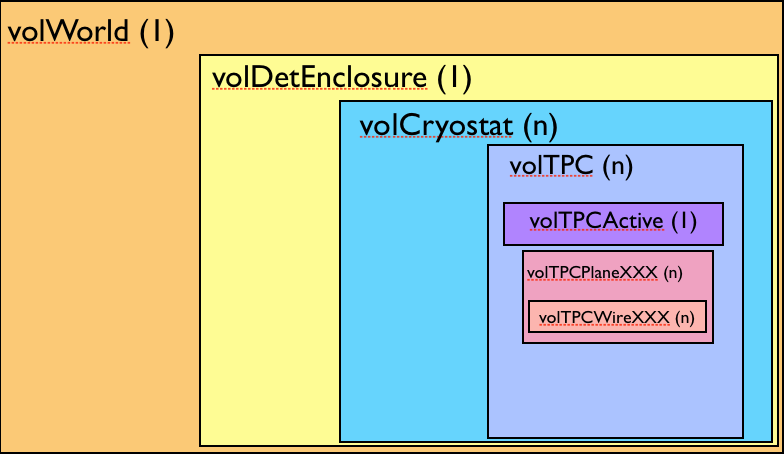
\includegraphics[width=4.0in]{./imgs/geometry_volumes.png}
\label{geo-vol.img}
\end{figure}

As shown in Figure~\ref{geo-vol.img},
the highest level volume is World which contains all elements of the geometry to be accounted for in the simulation and should be sized adequately to account for any features of the detector surroundings that are important for the simulation. For example, a huge mass of rock near the detector could alter the cosmic ray flux from that direction, it should be simulated. There is only one detector enclosure volume which can contain many Cryostat volumes, which can each contain many TPC volumes. Each TPC volume contains only one TPCActive volume, which defines the active volume of liquid argon that is read out by the detector. Any liquid argon that is outside of the drift field would not be part of volTPCActive. It is assumed that volTPCActive is simply a volume of liquid argon with no sub-volumes in it. 

The TPC volume contains many TPCPlaneXXX volumes that describe the wire planes. The TPCPlaneXXX volume contains many TPCWireXXX volumes that each describe a wire in the detector. The Geant4 binding and the ROOT binding support the GDML import and export for reading and writing GDML files.
                    
\section{Simulation Mechanics}

\subsection{Data Product Description}

\larsoft simulation jobs use the ART framework tools to manage job configuration, module scheduling and execution, error handling, and input/output. \larsoft simulation job modules perform the steps required for simulation. They communicate data from one job to the next via the event record in memory. The structure of the data within the event record is given by predefined data products, which are implemented as objects with C++ class definitions. If the data products required by downstream modules are saved in the output file of the upstream jobs, the steps required by simulation can be performed in separate jobs.

\larsoft-specific data products include:
\begin{itemize}

\item{the MCParticle which stores, per particle, a unique integer to index the particle in the list,}
\item{the PDG-recommended particle ID code~\cite{pdgcode}, }
\item{the counter number of its parent particle,}
\item{its mass,}
\item{the position and time of its starting point or of the first point to be simulated
for a particle entering from outside the active volume, and}
\item{its momentum and energy.}
\end{itemize}
A status code indicates which particles are to be simulated and which
are stored by the generator for extracting history and parentage as is the
case of $\pi^0\rightarrow\gamma\gamma$ decays, or particles that are absorbed within
nuclei.

The MCNeutrino data product contains a pointer to the MCParticle object for
the incoming neutrino, the outgoing lepton, and an interaction-type descriptor,
which indicates whether the event was a charged-current or a neutral-current interaction,
whether the struck nucleon was a proton or a neutron, what the recoiling system's mass is,
the Bjorken $x$ value, and the inelasticity quantity $y=E_\ell/E_\nu$.

The MCTruth data product is a container for the MCParticle and MCNeutrino
data products.  Some generators do not produce MCNeutrino objects, so MCTruth contains data members to indicate if the MCNeutrino information is filled in and to indicate the origins of particles.
 
The MCFlux data product stores information from the neutrino beam simulations. It has data members that mirror the G4NuMI ntuples, which provide information to reweight the flux from one model to another.

These data products are used as input to the LArG4 simulation step, described below. They are also indispensable in interpreting the events for later analysis, as MC samples typically contain mixtures of many different processes and energies. To determine the energy resolution for a specific kind of process or type of reconstructed event, it is important to know what the true values were.

The Geant4 physics simulation produces additional MCParticle objects, as simulated interactions
of particles with the detector material will produce additional particles.  These are stored in ParticleList.  Not every produced particle is stored in this way. Storing all 
particles in electromagnetic showers would require a large amount of storage with little contribution to physics. 
But storing the first few steps of an electromagnetic shower
is needed to characterize algorithms that separate showers initiated by electrons from those initiated by photons. So there are times when it is appropriate to loosen
the requirements on whether to accept additional particles for subsequent storage.

The detector response simulation data products are considered Monte Carlo truth-level information. The SimChannel data product accumulates information for each readout channel of the TPC, listing how many electrons drifted past it for the induction wires or were collected. Each of these charge deposits contains a total charge, a time, and an identifier of which Geant4 track was responsible for the charge deposition. The simulation of this charge is described in 
Section~\ref{sec:ionization}.

Similar to the TPC channel response truth information data products, photon detector truth information
is stored in the event record.  The SimPhotons data product stores information for each photon
that enters a sensitive OpDet volume.  It contains data members that specify the initial position of the
photon, as well as the time and the energy.    
This data product can be used with different photon detection technologies, such as detectors with wavelength shifting material covering the PMTs, and detectors with Silicon Photomultipliers (SiPMs) attached to wavelength-shifting materials and light collectors.

LArTPC detectors can have detector components in addition to the TPC wires and photon detectors.
For example, a detector may have external scintillator paddles, or other technology for external veto
counters.   A data product patterned after SimChannel is defined to store the MC information
for these auxiliary detectors.  Its data members store the Geant4 track ID, as well as the deposited energy, the entry and exit positions, and the time.

The goal of the simulation is to produce simulated data that matches what is expected from the detector for
the different input physics processes, along with detector resolution and noise effects.  These simulation
steps are described in Sections~\ref{sec:adapt} and~\ref{sec:ionization}. The output of this simulation is a vector of ADC counts,
one per sample time (typically 500 $ns$), for each readout channel in the detector.  Additional data members
store the pedestal and specify the compression algorithm type and version, such as Huffman coding or zero 
suppression. These are stored in a data product called RawDigit.

A similar structure is provided by OpticalRawDigit for the optical detectors, which read out
digitized waveforms with a much faster sampling rate, and in
AuxDetDigit for the auxiliary detectors.  OpDetPulse stores optical raw data only for 
subsets of the samples which contain identified pulses.

These data products are subject to modification as the requirements of the detector simulation evolve.
Large redesigns of a data product require new data product definitions, while
incremental updates can be accommodated in a backward-compatible fashion using ART's
data product schema evolution features.

\subsection{Adaptations for Using Geant4}
\label{sec:adapt}

The truth particles generated in the event generator step are passed to a Geant4 
based detector simulation called LArG4.  The geometry GDML file 
described in section~\ref{sec-geom-desc} is parsed to create a Geant4 detector description using
Geant4's GDML parser, which interfaces to \larsoft via the DetectorConstruction \larsoft class.
The following sections describe some features that distinguish
LArG4 from standard Geant4 simulations.

\subsubsection{User Action Lists}
\label{sec:useractions}
Geant4 includes several user-hook routines to modify Geant4's
standard processing. LArG4 makes use of Geant4's built-in hooks that
are called at the beginning and end of each event, track, and step to
record information related to the secondary particles created during
the detector simulation. These hooks are organized in the class
UserAction, which is part of the nutools package external to
\larsoft. UserAction uses a variant of the Abstract Factory design
pattern~\cite{designpatterns} to simplify the handling of multiple
simulation tasks, each of which might require access to Geant4's user
hooks.

The interface to G4Base/UserAction is implemented in the ParticleListAction routine 
which records the
information from each Geant4-generated secondary particle to create
the MCParticle data product. It returns a list of all such particles
created during a given event.
The basic algorithm records particle
information at the beginning of each track, and provides a readout
method to return the particle list at the end of each event. However,
there are a number of exceptions or enhancements:

\begin{itemize}

\item Geant4 assigns a unique ID number to every particle it tracks
  during an event: the track ID. At the start of a particle track,
  Geant4 provides a method call to determine the track ID of the
  parent particle for a given track, but there is no predefined method
  for determining the track IDs of any daughter particles produced by
  Geant4 as it models the propagation of the track through the
  detector. Therefore, the list of particles must be scanned at the
  end of the event to fill in the daughter fields of the MCParticle
  data product.

\item Geant4 can generate secondary particles down to a very low
  energy. This would result in a large number of MCParticle data
  products included in the output, with energies that are
  insignificant for reconstruction. Therefore, a threshold cut is
  applied via a job parameter to suppress the output of particles with
  kinetic energies below a certain value; the default value for this
  cut is 10$keV$. It is possible for a particle with kinetic
  energy that falls below the cut to generate a particle with energy
  above it; for example, an atomic nucleus may be excited and have low
  kinetic energy, then emit a decay particle with a kinetic energy
  above that cut. This results in orphan particles, that is,
  secondary particles in the output with no parent. 

\item For a large number of reconstruction studies, there is no need
  to store the daughter particles of electromagnetic showers. A job
  parameter controls whether particles produced in pair production,
  compton scattering, photoelectric effect, bremstrahlung,
  annihilation, or ionization should be included in the output. The
  default value of this parameter is to not include them. 

\item The MCParticle data product includes MCTrajectory that can cover the complete Geant4 trajectory
  information for a track. At each step within a particle's
  trajectory, the Lorenz four-position and four-momentum can be
  stored. This is useful for event displays and track-fitting studies,
  but is not needed for other studies such as energy
  calibration. Therefore, a job parameter controls whether or not the
  complete trajectory is stored for every MCParticle; the
  alternative is to store just the data for the first and last point
  of a particle's trajectory. The default value of this parameter is
  to store the trajectory.

\end{itemize}

\subsubsection{More User Actions}
\label{susubsec:trackstackingandeventbiasing}

The statistical errors on rare event studies in \larsoft can be improved via track stacking and event biasing.

The priority of Geant4 tracking within a simulation defaults to stepping through certain tracks
until their final fates are determined. This is done 
by tracking a particle until it decays, exits the world volume, drops below a kinetic
energy cut, or annihilates. It may be desired to suspend or stop 
the tracking of a particle and instead track a daughter of an interaction. 
This occurs when pursuing a cosmogenic study in which muons need to be tracked in 
the non-instrumented volume of material surrounding the actual detector, but the real concern is the penetration of daughters into the instrumented detector. If the muon initiates an inelastic interaction and then falls below 
an energy that's likely to produce another such interaction and/or it is kicked in a direction that makes
it unlikely that any further daughters would make it to the detector, it is wise to
track any daughters of interest from this interaction and abandon or at least delay the tracking of the incident muon.
If the tracking is delayed, Geant4 will return to it later in the event or in a subsequent event. If the muon is very far from the active detector after some amount of tracking, the tracking can be stopped or the event killed. This saves valuable processing time since it provides movement
immediately onto the next candidate event that might give activity in the detector.

Track stacking is done in \larsoft by defining an optional post-step class 
called LArStackingAction that derives from UserStackingAction. It is instantiated and used upon proper setting of the desired 
FHICL job flag. In addition to the ParticleListAction 
described in Section~\ref{sec:useractions}, LArStackingAction is called at each step.
A status is assigned to all 
tracks after the step of interest in a 
newly implemented virtual method of the derived UserStackingAction class. 
Tracks may be assigned the status of
postpone, waiting, kill, or urgent. Geant4 will switch from its internally decided priority (usually to continue tracking the mother particle) to track the new particles that
the user has determined to be higher priority. 

Event biasing is needed to explore infrequently occurring physics processes since it may
not be enough to just dictate what to track in which order. Rare interactions in Geant4 may be made to occur with higher 
probability than their naturally-dictated rate by artificially increasing their cross-sections. The cosmogenics example mentioned above is 
aided by two related strategies to produce the interaction of interest in the detector
with higher probability than occurs naturally. It is also possible to generate multiple outgoing daughters rather than whatever the low natural
number may be. This requires careful tracking of the weights of any new 
particles introduced. This is done in \larsoft by writing physics classes which are processes obeyed by particular particles derived from the G4WrapperProcess. Secondaries are generated 
and weights are calculated for all the G4Particles. These are preserved and passed down all the way to \larsoft's MCParticles.

Without a combination of track stacking and event biasing, statistical errors on rare event studies would dominate due to the few events of interest that may result even after large batch submissions.

\subsubsection{Readout Geometries}
\label{sec:detsim}

The basic purpose of the Geant4 simulation of a LArTPC detector is to
model the ionization left by charged particles created by interactions
in the detector. This information is easy to retrieve using the
standard Geant4 method GetTotalEnergyDeposit. The next
step in the process is to convert that ionization into electron
clusters and drift them to the wires of the induction and collection
planes. 

The ionization deposited by a charged particle is not necessarily
constant along the entire length of a charged-particle track. To
accurately convert the ionization to electron clusters as described in
Section~\ref{sec:ionization}, it is necessary to divide the track into
short segments and apply the ionization procedure to each segment
individually. There are two ways to approach this in Geant4:

\begin{itemize}
\item Set the Geant4 step size to a small value for charge-particle tracks in the LArTPC.
\item Divide the LArTPC into smaller sub-volumes, which will force Geant4 to limit the step size to the boundaries of these volumes.
\end{itemize}

The second approach is taken in LArG4. This procedure permits LArG4 to
sum the total amount of ionization energy deposited in each
sub-volume, called a voxel in analogy with the word pixel, the
term for a small area of a two-dimensional image. This allows
corrections for potential saturation of the liquid argon within the
voxel, which would be difficult to determine in the first approach.

The ${\Delta}x$, ${\Delta}y$, and ${\Delta}z$ dimensions of the voxels
are given by user parameters. By default, they are 1/10th the spacing
between the wires of the induction and collection planes in
MicroBooNE; the wire spacing is 3$mm$, hence the default voxel size is
$0.3mm\times0.3mm\times0.3mm$. There is also a ${\Delta}t$-component
to voxel processing, intended for potential overlay studies; in
practice it is not used, and is set to 5${\mu}s$.

The voxel readout geometry does not physically exist, and so it is
implemented using Geant4's parallel world mechanism. Geant4 tracks
particles through the regular geometry and any parallel geometries
simultaneously, limiting steps within the volume boundaries in all of
them. This is further refined in the PhysicsList routine,
which specifies that only charged particles are to be tracked in the
parallel voxel geometry (since only charged particles deposit
ionization energy). (Note that the voxels described in 
Section~\ref{sec:fullopticalsim} are defined separately in yet another
parallel geometry, and share no characteristics with the voxels
described in this Section.)

In LArVoxelReadoutGeometry, a copy of the LArTPC geometry
is placed in a parallel world, then subdivided into voxels; each voxel
is defined to be a Geant4 sensitive volume. As Geant4 tracks charged
particles through the parallel voxel geometry, it calls the
sensitive-detector routine LArVoxelReadout. The ionization
is then converted into electron clusters as described in
Section~\ref{sec:ionization}.

Each SimChannel
data product contains a link between an electron cluster and the
Geant4 track ID of the ionizing particle that was its source. However,
if a particle's kinetic energy falls below the user cut described in
Section~\ref{sec:useractions}, that particle's track ID will not be in
the group of MCParticle data products output by the
simulation. It is therefore possible to have orphaned energy, that
is, electron clusters that cannot be associated with a particle in the
output. 

The most common reason for orphaned energy is that the MCParticle
was not written because it was the daughter
particle of an electromagnetic shower, and the user has chosen not to
include these particles in the LArG4 output. Therefore, LArVoxelReadout calls a method in ParticleListAction to query the current track ID. If the
particle is part of an e-m shower, rather than returning the current
Geant4 track ID, ParticleListAction responds with the
track ID of the particle that induced the e-m shower, which is the
particle normally of interest in shower reconstruction studies.

\subsection{Adding Additional Detectors}
Other types of detectors may be placed outside of the cryostat volume.
For example, scintillator paddles or Cherenkov detectors could be used to learn more about an interaction happening in the cryostat.
Scintillator paddles could be used to veto cosmic ray activity or hadronic showers coming from a neutrino beam interacting with material upstream of the detector enclosure.
Cherenkov detectors could be used to measure the velocity of incoming particles from a test beam used for studying liquid argon TPC responses.
A new object was created in \larsoft to allow users to store general information from detectors not related with the TPC, or auxiliary detectors.

For each Geant4 track passing the auxiliary detector volume, the \larsoft object AuxDetSimChannel holds its entering and exiting position, momentum, energy deposited, and \larsoft track ID.
That information is saved for each auxiliary detector in the output root file.
This data object allows the use of the Geant4 track ID to trace back the genesis of a particle crossing the detector, enabling simulation studies and efficiency studies of external auxiliary detectors.

To add new auxiliary detectors, the user needs to define the detector in the experiment's GDML file.
\larsoft has a facility to identify those volumes to enable Geant4 to treat them as an active detector.
As Geant4 encounters a new Geant4 track ID within the active detector, the AuxDetSimChannel data object stores each entry position and entry momentum.
While Geant4 steps through to the next time slice, each particle's exit position and exit momentum is updated, and the running sum of energy deposited is updated. 
After the Geant4 steps are exhausted for this detector, the AuxDetSimChannel object has collected all of the simulation data needed for further analysis.

\subsection{New Parameterizations for Ionization}
\label{sec:ionization}
- description of how new parameterizations for ionization, etc can be added into the simulation including a description of the mechanism for calculating the amount of ionization charge and scintillation light.  It could include a statement of the available options for that calculation (NEST vs decoupled charge and light) and how a user might add a new method.~\cite{nest}
NEED WORDS

\subsection{Incorporating Magnetic Fields}
\larsoft provides limited support for simulating magnetic
fields. A constant and uniform field may be specified
throughout any single volume (and it's sub-volumes) of the Geant
geometry, and will be respected by Geant's particle tracking
algorithms. There is currently no support for altered electron
drift directions, nor any explicit support for analyzing events
in the presence of a non-zero magnetic field although both of these features are planned.

\subsection{Optical Simulation}
Optical physics simulations in \larsoft can take one of two forms: full or fast simulation.  Both optical simulations are implemented within \larsoft's Geant4 based simulation package and make use of its configurable physics list functionality.  This functionality allows \larsoft simulations to define a custom Geant4 physics list from a set of physics constructors at runtime, and is used to select between full optical, fast optical or no optical simulation. 

\subsubsection{Full Optical Simulation}
The full simulation involves stepping individual photons through the detector volume.  Each stepping photon is treated as an individual particle in Geant4.  The number of photons stepped is usually reduced by a constant factor representing the optical detector collection efficiency at 128 $nm$, thereby scaling the photon count at production rather than detection to reduce computation time and memory usage. 

The physics constructor for full optical physics in \larsoft has been adapted from the standard Geant4 optical physics constructor. Default implementations for scintillation and Cerenkov production, Rayleigh scattering, and absorption at boundaries and in the bulk are included. The default implementation of wavelength shifting physics processes is also included, although at present most \larsoft experiments incorporate this into the estimate of the optical detector collection efficiency rather than simulating it at the photon-by-photon level.  A customized, faster reflectivity model is implemented, whereby material boundaries have specified diffuse and specular reflectances for each material boundary type.  

The liquid argon volume's optical characteristics are loaded into \larsoft by a dedicated service, and are globally accessible within the \larsoft framework.  Reconstruction and simulation algorithms can access important optical properties.

Scintillation production is configured with a photon momentum spectrum centered at 9.7 $eV$ and a shape which is taken from~\cite{spectrum}.  Singlet and triplet scintillation components are included, with time constants of 6 and 1500 $ns$, although tensions within the literature suggests these values will require finer tuning.\cite{fastslow}\cite{fastslow2}\cite{fastslow3}\cite{fastslow4}
Data from \larsoft experiments will be used to adjust these values.  The scintillation yield is defined per incident particle type using an extension of the relationship shown in~\cite{scintyield}, and the absolute yield for a minimum ionizing particle is set to 24,000 photons per million $eV$, assuming a constant electric field strength of 500 $V/cm$. 

Cerenkov photons are produced with yields and energies corresponding to the standard Frank-Tamm spectrum of Cerenkov radiation, given a continuous parameterization of the liquid argon refractive index derived from the references in~\cite{RIndex}. Rayleigh scattering and photon-absorption process are enabled, where the scattering length is specified over the range of photon energies from 1.8 $eV$ to 10.8 $eV$, and is 90 $cm$ at the peak of the argon scintillation spectrum~\cite{Rlength}.  The bulk absorption length is set to 2000 $m$ (approximately infinite). Further work to parameterize purity dependent absorption effects may be required, with absorption due to dissolved nitrogen being the most likely additional effect~\cite{nitrogen}.

\label{sec:fullopticalsim}
The full simulation involves stepping every optical photon individually through the detector volume.  Typical photon yields for an event cause this to be a computationally intensive procedure. The physics constructor has been specially adapted for \larsoft and includes scintillation and Cerenkov production, Rayleigh scattering, reflections at boundaries, absorption at boundaries and in the bulk, and wavelength shifting physics processes.

A simplified reflectivity model is used, whereby each type of boundary in the detector is supplied with a wavelength-dependent total reflectivity and specular/diffuse reflection fraction.   For  preliminary  studies,  only the  steel/argon boundaries  at  the  edge of the cryostat are  reflective. All  other  surfaces,  including  wires,  field cage,  etc,  are opaque.  The steel/argon boundaries have a total reflectance of 25\%, of which 50\% is specular~\cite{reflectances}.

\begin{figure}[h]
\centering
\caption{Illustration of the simple treatment of wireplane absorption in \larsoft}
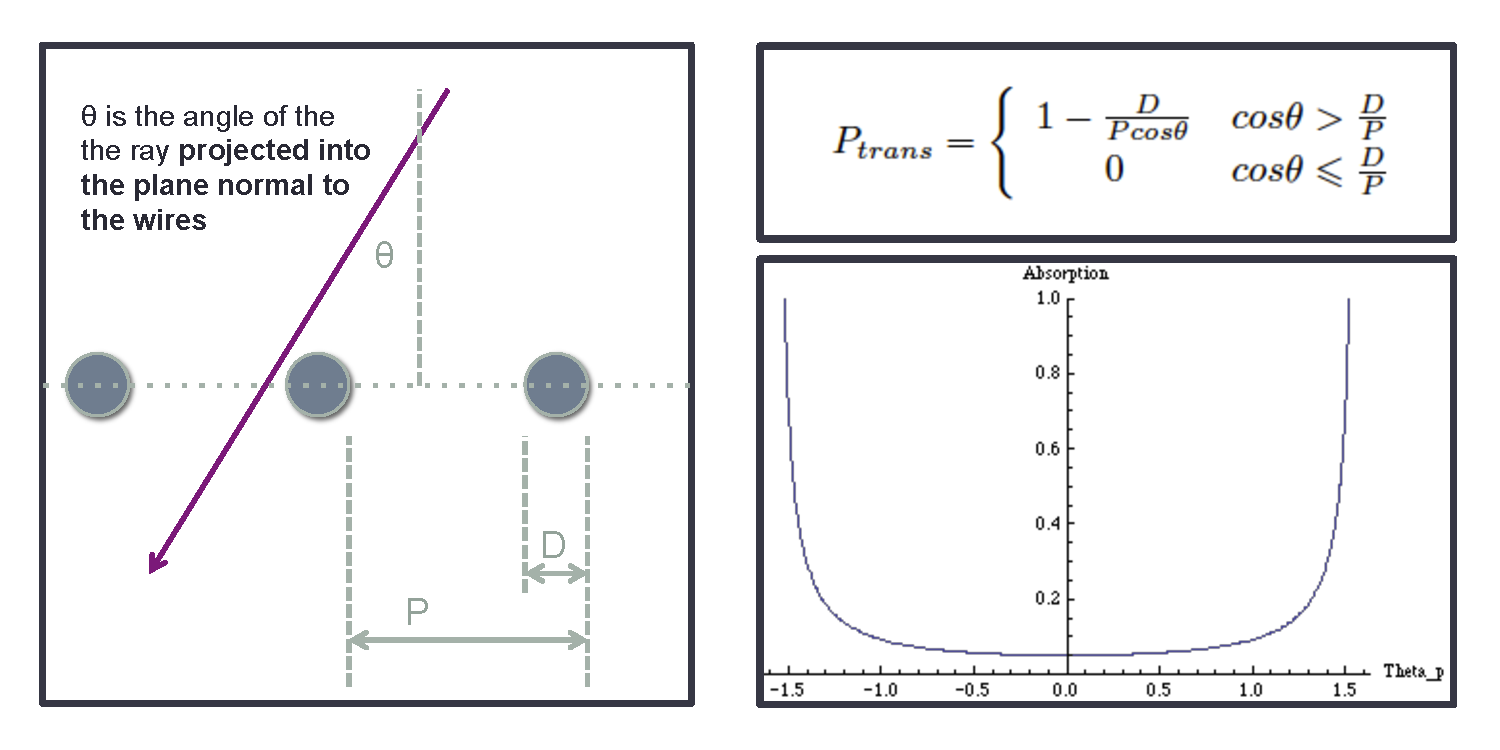
\includegraphics[width=6.0in]{./mtrls/imgs/WireplaneTransmissionCartoon.pdf}
\label{fig:wireplaneabs}
\end{figure}

For a given surface, any angularly dependent transmission spectrum can be incorporated, including semi-transparent surfaces.  Non-uniform angular dependence of photon transmission can be modeled through the detector wireplanes.    \larsoft derived classes implement optical attenuation by one or many planes of cylindrical wires which are assumed black to 128 $nm$ light. A cartoon of the wireplane opacity model is shown in figure~\ref{fig:wireplaneabs}.

Photons are counted at detector volumes whose name matches a string supplied to the \larsoft geometry service.  This volume may represent a photomultiplier tube, or another element defined as optically sensitive, for example, a wavelength shifting surface. At geometry construction time, the volumes matching the appropriate name string in the GDML file are assigned optical detector IDs and become sensitive within the \larsoft simulation.

Three parallel world geometries are used in \larsoft as shown in figure \ref{fig:parallelgeom}.
The sensitive elements are placed in a separate Geant4 parallel world geometry.  Only photons are tracked in this geometry, ensuring the optical  detection process is triggered only for optical photons.  Photon step size is not limited by the TPC voxel size, which provides a significant performance improvement. Upon photon detection, tracking of the photon is stopped. Information about the photon's arrival time and detection location are stored in a detected photon table.  At the end of the run, this table is queried to generate simulated photon data products to store in the event.  The same table is filled by the fast simulation method, and hybrid fast and full simulations can be run.  One use case for such a hybrid simulation would be the fast simulation of scintillation photons. Full simulation is required for Cerenkov photons, which have a directionality and so cannot be consistently treated by the fast simulation.


\begin{figure}[h]
\centering
\caption{A cartoon which illustrates the three parallel simulation geometries used in the \larsoft
Geant4 implementation.}
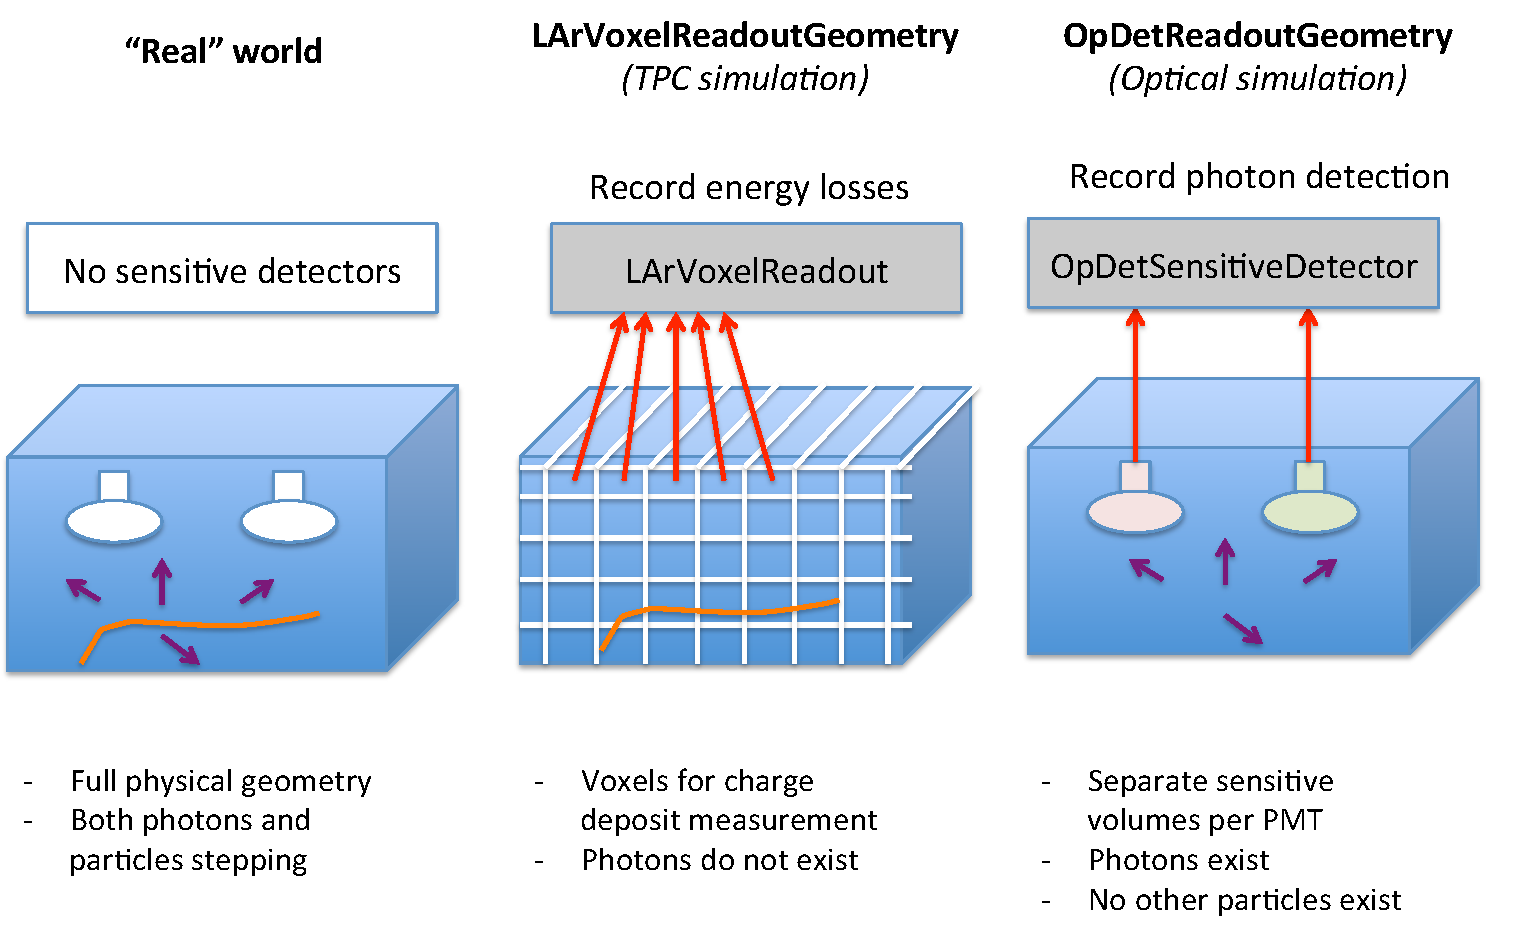
\includegraphics[width=6.0in]{./mtrls/imgs/ParallelGeomScheme.pdf}
\label{fig:parallelgeom}
\end{figure}

\subsubsection{Fast Optical Simulation Modules}

The number of optical photons generated per event is of the order of tens of millions per GeV, so full optical simulation is a computationally intensive process.  Since scintillation in argon is isotropic, the visibility (defined as the fraction of generated photons which will reach a given optical detector) can be pre-calculated at each point in the detector.  The fast optical simulation uses this approach to avoid stepping individual photons during routine simulation jobs.

The liquid argon volume of the detector is coarse-grained into optical voxels, the size of which must be smaller than the resolution of the optical system but can be significantly larger than the TPC voxelization scale.  The optical fiducial volume incorporates all detector volumes which are visible to the optical system, which in general extends further than the TPC fiducial volume.  The complete cryostat volume is optically voxelized by default. If there are invisible regions for a specific detector, a smaller optically active volume can be specified.

A dedicated run of the full optical simulation can be made to create a lookup table which contains the visibility of each voxel to each optical detector.  This run creates a specified number of isotropic 128 $nm$ photons, uniformly distributed across each voxel volume at time t=0.  These photons propagate and are detected using the same mechanics as the full photon simulation.  After photon propagation, the number of detected photons at each optical detector is used to build the optical visibility lookup table.  This process is automated by a dedicated photon visibility service, which communicates with the event generation, simulation and analysis parts of the simulation chain to ensure they are correctly configured.

Once the visibility table has been generated, the probability that a given 128 $nm$ photon will reach a specified optical detector can be quickly assessed using the photon visibility service which is available to both simulation and reconstruction modules.  The \larsoft Geant4 simulation can be configured to include the fast optical physics constructor which implements the lookup-based fast scintillation process within simulations. The generation parameters for scintillation light in the fast scintillation process are equivalent to those used in the full simulation.  However, instead of placing optical photons onto the Geant4 particle stack, detected optical photons are inserted directly into the detected photon table probabilistically, based on the visibility of the detector location where the scintillation occurred.  The arrival times of the photons are also smeared based on the distribution of production times.  The sum of detected photons from each voxel where scintillation emission occured gives the total optical detector response.

The photon library is both geometry and voxelization scheme specific, and changes to either require a full regeneration, which is a computationally intensive job.  The effects of Rayleigh scattering and absorption are also built into the visibility table.  Changes to the argon scintillation production properties and optical detector efficiencies can be made without regenerating the table.

\subsubsection{Tools for Optical Simulations}

There are several tools in \larsoft used for optical simulation validation and basic analysis.  The photon counter module produces analysis trees and histograms representing the properties of the detected photons in each optical detector.  The module extracts per-optical-detector and per-event information for both full and fast simulation outputs.  It is also used to generate the optical visibility library used by the \larsoft fast simulation.

\begin{figure}[h]
\centering
\caption{An example of slices through an optical visibility table. This shows the visibility at various points
in the MicroBooNE detector.  This plot was made from the optical visibility table using the optical library
analyzer module.}
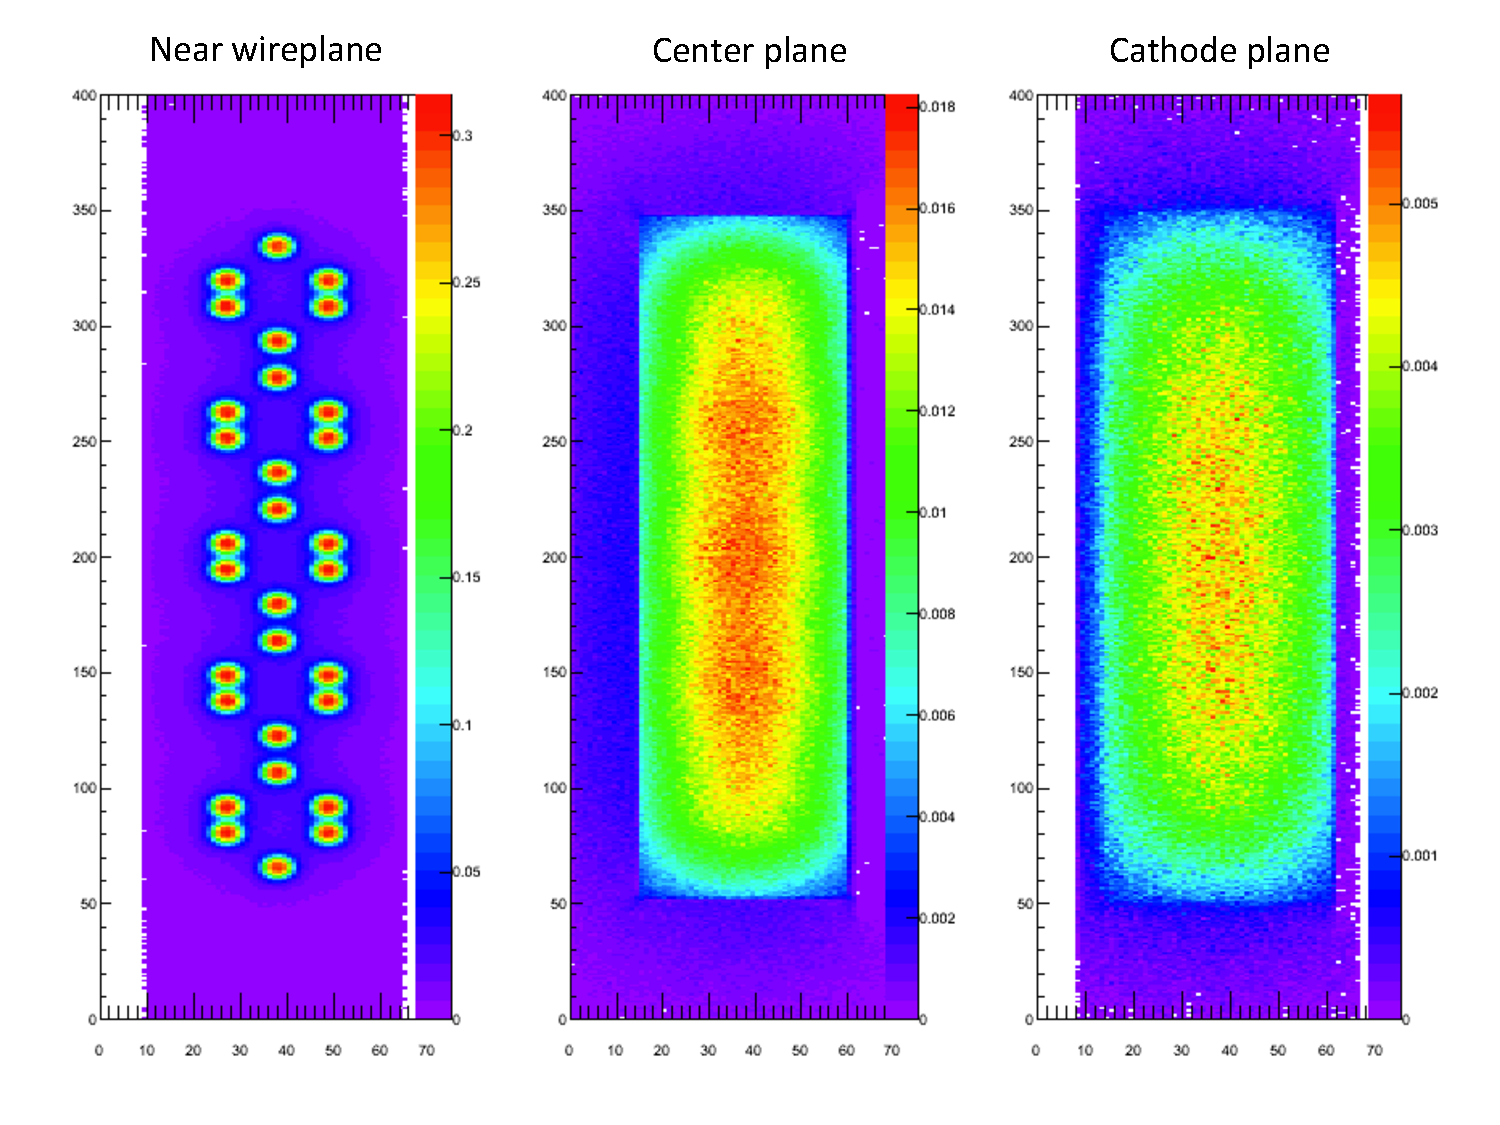
\includegraphics[width=6.0in]{./mtrls/imgs/SampleOpticalMap.pdf}
\label{fig:opticalmap}
\end{figure}

The light source event generator can be configured to generate photons at a specified wavelength and with a specified geometry and time.  The light source can be configured to step through each optical voxel event-by-event, or else to step through a custom set of arbitrary geometrical configurations specified in a text file.  This event generator is particularly useful for investigating the optical response to different event geometries and is used in the generation of the photon visibility library.

A library analyzer module produces detector visibility maps and other histograms based on the loaded visibility library.  This module is used to validate the optical library and obtain information about the detector response to light deposits at different points.  Some histograms produced by this module for the MicroBooNE optical library are shown in figure \ref{fig:opticalmap}.


\section{Reconstruction Mechanics}

The \larsoft reconstruction is highly flexible due to the design principal it employs of requiring all algorithmic steps of the reconstruction to be encapsulated into individual objects.  Those objects can in turn be called in a variety of combinations that allow a user to move from basic raw data to very high level reconstruction.  These algorithm objects are consolidated into modules that are called by the framework to produce the desired data products.  The modules can perform a single step of the reconstruction or multiple steps, but are all required to produce data products that need no further processing to be handed off to another reconstruction stage or an analysis stage.  As a result of this feature, the user has a high degree of discretion to design a reconstruction path that seems appropriate for the desired application.  For example, one user may choose to build up a set of two dimensional reconstructions to combine into a three dimensional one, while another user may opt to attempt a three dimensional reconstruction directly from the energy depositions of the raw data.  

\subsection{Data Product Description}

The \larsoft data products for reconstruction are designed to provide descriptions for the various stages of and approaches to the reconstruction.  The data products describe both two dimensional concepts, such as which energy depositions are closely correlated in both time and space, as well as complicated three dimensional concepts such as which particle tracks and showers should be combined to describe a single particle interaction in the detector.

The \larsoft data products that describe two dimensional concepts are the Wire, Hit, Cluster, and EndPoint2D.  The Wire describes all information from a single calibrated channel of the detector.  It is intended to be an intermediary between the raw signal of the RawDigit object and the rest of the reconstruction.  The user may choose to save the Wire objects to the resultant output file of a reconstruction task, but that is not required.  The Hit encapsulates the concept of a single energy deposition on a single channel in the detector and contains information about the electronics channel recording the hit as well as the magnitude of the deposition.  The Cluster is the association of all Hits that are correlated with each other in space and time.  The EndPoint2D represents an end of a line-like cluster or the start of a diffuse, shower-like cluster.

The data products that describe three dimensional concepts are the SpacePoint, Seed, Track, Shower, Vertex, Event, and PFParticle.  

\subsection{Organization of Algorithms}

What is an algorithm? How do they relate to modules?

\subsection{Implementation Plan for Algorithms and Modules}
NEED WORDS.

\subsection{Unique aspects of \larsoft Reconstruction}

\subsection{One Example Reconstruction Chain in \larsoft}
The reconstruction chain used by the MicroBoone experiment to reconstruct cosmic and neutrino interactions is described as follows.

\subsubsection{Signal Shaping}
A LArTPC typically saves raw data in the format of ADC counts as a function of TPC ticks for each wire. The signal can have a unipolar shape if it is on a collection wire or a bipolar shape if it is on an unshielded collection wire. The first step in the reconstruction is to convert the raw signal from each wire to a standard shape such as a Gaussian shape. This is achieved by passing the raw data through a calibrated deconvolution algorithm, which filters noise and corrects for the electronics response and the effect of the drift field response to produce the best estimates of the drift charge and time. 

\subsubsection{Gaussian Hit Finder}
Gaus(s)HitFinder (initially checked into the code repository with a mis-spelling in the title and henceforth was embraced as the intentional spelling) is a hit-finding algorithm used as the primary hit-finding algorithm in ArgoNeuT and MicroBooNE experiments. The algorithm works starting from deconvolved signals on wires and and defining areas above threshold known as ``pulses''. Once a pulse is found, a `n' Gaussian hypothesis is applied where `n' is defined by the number of peaks initially identified within the pulse. Based on the outcome of the fit and object known as a ``hit'' is formed and stored on the event.

\subsubsection{Fuzzy Cluster}

After hit finding has completed, the hits in each plane are clustered. The goal of a clustering algorithm is to categorize hits into individual physics objects as best as possible in 2D. Fuzzy Cluster is such an algorithm and proceeds in five stages.
\begin{enumerate}
\item
The first stage implements the FLAME clustering algorithm originally developed for the analysis of DNA microarray data~\cite{flame}. The goal of the FLAME clustering algorithm is to break hits on the selected plane into smaller portions to improve memory usage of the second step, the Hough transform. 
\item
The Hough transform identifies hits that form line-like objects such as tracks. The particular variant of the Hough transform implemented is the Progressive Probabilistic Hough Transform, which is optimized for speed and light memory usage~\cite{ppht}. 
\item
After lines have been identified in the collection of hits, a set of line merging steps 
group hits included in the identified lines into track-like and shower-like objects.
\item
The hits not incorporated in lines by the Hough transform are merged into the nearest cluster formed from the identified lines. The hits are only merged with lines provided they satisfy a distance requirement. 
\item
The final step runs the DBSCAN clustering algorithm, described in~\cite{dbscan}, over hits that were not incorporated into lines from the Hough transform or merged with hits already part of a line. 
\end{enumerate}


\subsubsection{Track Kalman Filter}

The track reconstruction problem in a liquid argon TPC can be
divided into several stages, including pattern recognition
(identifying hits that belong to a track), trajectory reconstruction,
and track parameter estimation. Although in principle tracks can be two or
three-dimensional objects, \larsoft uses only three-dimensional
tracks.

Hits are the input data for track reconstruction.  Hits
represent a one-dimensional measurement of a track (the
drift time) on a measurement surface defined by the charge drift
direction and the readout wire. Two or three hits may be combined
into three-dimensional space points. Three dimensional track
reconstruction can proceed from space points or directly from hits.

The Kalman filter algorithm~\cite{kalman} has been widely used in high
energy physics for track reconstruction. The Kalman
filter provides an elegant mathematical solution to the problem of
finding an optimal track description from a collection of candidate
measurements that are hits or space points, especially in cases where the
number of measurements is much larger than the five parameters
needed to specify a track on a surface.  The Kalman
filter can be used for both pattern recognition and parameter
estimation.  Furthermore, the Kalman filter in \larsoft can use either hits or
space points as input.

The following is a description of the basic Kalman filter algorithm.

\begin{enumerate}
\item
Starting from an initial track estimate, generate a predicted
measurement (hit or space point) and error on the next measurement
surface.
\item
Use the predicted measurement and error to define a road for selecting
candidate measurements.
\item
Use the road defined in the previous step to select hits for inclusion
in the track.
\item
Use the included hits to refine the track estimate.
\item
Repeat steps 1--4 until all candidate measurements are included in the
track or rejected.
\end{enumerate}

The skeleton Kalman filter requires qualifications and caveats in real cases. The remainder of this
section describes some of the qualifications that apply to the
hit-based Kalman filter in \larsoft.

The Kalman
filter algorithm is not self-starting. That is, an initial estimate
of the track parameters is required even for the first time.  In the \larsoft hit-based Kalman filter, the initial
estimate of track parameters is provided
by a separate seed-track finder. Seed tracks are
collections of hits from all views that are reconstructed to form a
short straight three-dimensional track segment. The seed-track finder
is based on a Hough line finder~\cite{ppht} that finds straight track
segments in each view, and then combines 
Hough lines that are consistent in position and angle from different views into three-dimensional
objects.

In the initial
stages of reconstruction, when the track contains only a few hits, the
track parameters errors are very large. The Kalman parameter update in
step four can easily force the track parameters out of the range of
validity of a quadratic approximation of the chisquare function
between track and hit.  For example, the track direction may be
perturbed by the Kalman updating equation so that the
track reverses direction in one or more views.  To prevent
this, in the early stages of track reconstruction, the hit Kalman
filter uses a linearized propagation model that forces the chisquare
function to be a perfect quadratic form with a minimum close to the
seed track parameters.  This ensures that the Kalman filter will
generate a track close to the seed track in the initial stages of
reconstruction.  After the track parameters are sufficiently small,
the linearized approximation is abandoned, and the true propagation
function is used.

The measurement surfaces in liquid argon TPCs are intersecting, which means there is no
predetermined order in which the measurement surfaces should be
visited.  To prevent back-and-forth tracking, which would overestimate
propagation noise, such as multiple Coulomb scattering, the \larsoft
hit Kalman filter chooses the measurement surfaces associated with one
view as primary, and visits these surfaces in their natural
predetermined order.  Hits from views other than the primary view are
added to the track by treating the propagation from the track surface
to the non-parallel hit measurement surface as part of the measurement
function.  This measurement propagation is always done using a linear
approximation as is the measurement function, and is done without
propagation noise.

The \larsoft hit-based Kalman filter
does not use a branching track model. Hit selection (step two) for the \larsoft hit-based Kalman filter is
implemented such that at each measurement surface, the filter accepts
either zero or one hit. If the Kalman filter accepts a wrong hit, the
track may follow the wrong road (e.g. a delta ray), or the track may
otherwise end prematurely.  Fixing broken tracks relies on
a track-stitching algorithm that runs after the initial Kalman
filter reconstruction.

\subsubsection{Calorimetry and PID Reconstruction}
[Calorimetry and PID - Tingjun]

\subsubsection{Shower Reconstruction}

The electromagnetic shower reconstruction code happens in two steps. The first is a post-clustering stage which examines the existing clusters in terms of their 2D parameters to determine whether the clusters are shower-like or track-like. The user has the possibility of refining the existing clusters by additional merging steps before the final shower-track decision. The selected shower-like clusters are examined to determine their exact starting point, direction and angle in the wire-time plane. These parameters are passed on to the second step, the 3D shower reconstruction code. At this stage, the 2D clusters are matched between the views to obtain at least one cluster in two views per tentative shower. These sets of 2D clusters and their 2D angles and start points are then used to construct the 3D shower axis and start points via trigonometric formulae. This allows the calculation of the shower energy and charge deposition at the start of the shower used in particle identification. The start point, 3D angle, energy and $dE/dx$ values are then saved on the event stack for use by an event builder.

\subsubsection{PANDORA Reconstruction}
[PANDORA - Andy]
\subsubsection{Optical Reconstruction}
[Optical - Wes]

\subsection{Event Visualization}
An important part of the \larsoft suite is the ability to visually display events. The basic event display is constructed based on ROOT GUI libraries~\cite{ROOT}.
It can be used to display both data and MC events at any stage of their reconstruction, the latter with the corresponding MC truth information. 
Navigation between events is either by inserting the desired run and event number in the corresponding fields or by means of the next and previous buttons.

The basic event display window, figure~\ref{2d_event} shows projections in wire-time space for each of the views present in the given detector, where the quantity of charge in ADC collected in each wire is denoted by a color scale or intensity of gray-scale. The ADC threshold of what is displayed is a settable parameter. 
The user has the option of overlaying an MC event with the MC truth tracks color coded by particle type. The main display window is completed by a wire viewer, which shows the time series of a selected single wire in any of the views; the displayed wire can be chosen via mouse click or a field entry window.
All of the above pads have zoom capability. The user can choose what reconstructed objects are displayed, and which module created them, by using a special menu window or by specifying this in the FHICL configuration file at runtime. 

The event display has additional windows that allow different visualization of some of the reconstruction objects. These include the 3D event display, as shown in figure~\ref{2d_event} where the 3D Track objects can be viewed in a 3D depiction of the detector, a set of 2D projection views where the tracks are shown in the X-Z and Y-Z plane instead of the wire-time views, and a Calorimetry view where the track and Shower dE/dx depositions are plotted against MC predictions allowing visual particle identification. 

Since the event display is a \larsoft module, it can be run in sequence with other modules. It is possible to change the FHICL parameters of other modules running in the same job via a menu window. Using this capability and seeing the results of these changes in the event displays is a useful debugging tool in algorithm development.


\hspace*{2cm}
\begin{figure}[h]
\centering
\caption{Event display window}
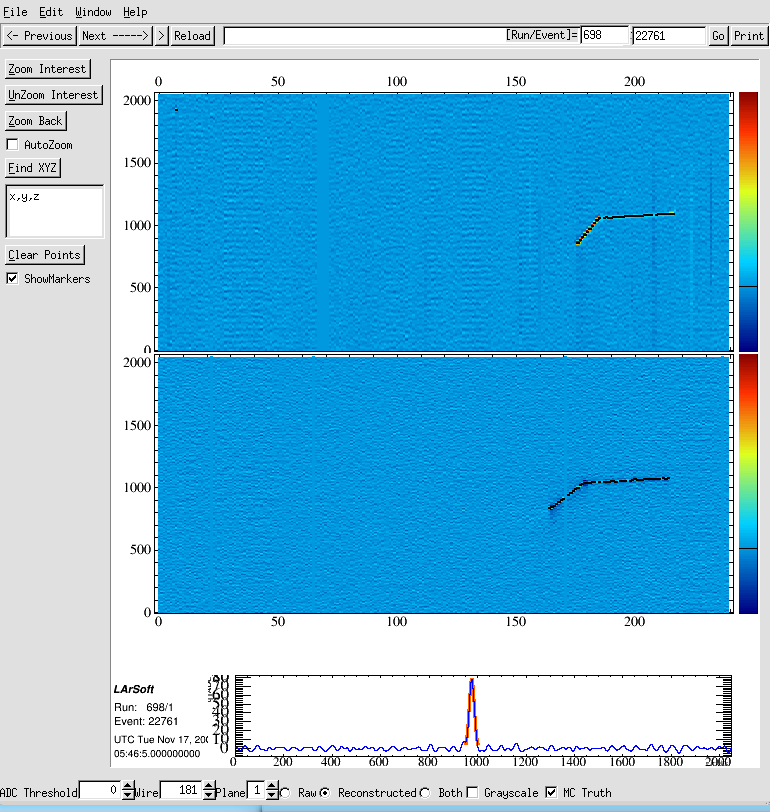
\includegraphics[width=4.0in]{./imgs/larsoft_2d_event_display.png}
\label{2d_event}
\end{figure}

               
\section{Analysis Mechanics}

\subsection{Data Product Description}
NEED WORDS.

\subsection{Organization of Algorithms for Analysis}
NEED WORDS.

\subsection{Implementation Plan}
NEED WORDS.

\subsection{Unique Analysis Aspects of \larsoft}
NEED WORDS.

\section{Getting Software and Benchmarking it}
\subsection{Ways to Contribute}

\larsoft general software is hosted in ten Git repositories with additional experiment-specific repositories for other source, for example digitization code and configuration files. MultiRepository Build (MRB) compiles code across Git repositories. Each repository has a test area, a documentation area, and libraries such as EventGenerator, LArG4, HitFinder, VertexFinder, etc.~\cite{gian}

To avoid having one developer's code negatively impact other software and to allow for vetting before others use the new software, no development takes place directly on the develop branch of the repository. \larsoft uses the git-flow~\cite{git-flow} model which makes it easy for users to have a private version of the software they are working on. This model allows the user to manage different tasks at the same time, each in its own independent branch, developing and testing code while sharing it with other users.~\cite{git-control} All \larsoft developers are expected to follow this workflow model to maintain the integrity of the develop branch.

A group of people, the librarians, vet the code going into all releases. The librarians may examine the changes made to the software in detail as well as looking at the bigger picture to ensure the software module performs the expected task(s). In particular, they ensure that the new code does not negatively impact other \larsoft software. Librarians also ensure the new code is documented and that tests are provided.

Librarians interact with the authors until the code meets the tenants listed at~\cite{code-tenants}. \larsoft code is intended to be usable by Liquid Argon TPC with any number of planes, wires, or PMTs. In addition, the code should be flexible and well-documented. 

\subsection{Testing}

In \larsoft, there is unit testing and integration testing which includes regression tests. Unit tests check very small parts of the code and are run by the author of the code. 
The integration tests are written by the author of the algorithm or feature that they test. These tests may be executed by other people in the project as well as the author. It must be possible to automatically run unit and  integration tests.

\larsoft has set up a Continuous Integration system based on Jenkins~\cite{jenkins} that routinely performs a sequence of tests including unit tests, integration tests and regression tests. On failure, the automatic system notifies \larsoft personnel who contact the responsible person(s), e.g. code authors or librarians, to fix the error.

\subsection{Resource Usage}

A rough estimate of resource usage can be obtained by running standard ART services called TimeService and SimpleMemoryCheck. TimeService gives an estimate of the time used by the module to perform its task. SimpleMemoryCheck monitors the usage of memory (RAM) by the whole program. In order for jobs to run smoothly in a GRID or remote environment, the job should use less than 2 Gigabyte of memory, and less than 48 hours of CPU time.

A resource coordinator in \larsoft checks for excessive usage, and if found, analysis is done using tools like Valgrind~\cite{valgrind}, Gperftools~\cite{gperf}, and Allinea.~\cite {allinea}.
The code author is notified by the resource coordinator of the issue and together they develop a solution to the resource problem. Most typical problems relate to the use of data structures, and can be solved by following the ART guidelines.~\cite{art-guide}
 
\section{Summary}
NEED WORDS.
\section{References}

\begin{thebibliography}{99}

\bibitem{art-ref} https://cdcvs.fnal.gov/redmine/projects/artdaq
\bibitem{cry} http://nuclear.llnl.gov/simulation/
\bibitem{genie} C.Andreopoulos et al., The GENIE Neutrino Monte Carlo Generator, Nucl.Instrum.Meth.A614:87-104,2010.
\bibitem{nuwro} Tomasz Golan, Cezary Juszczak, Jan T. Sobczyk. ``Final State Interactions Effects in Neutrino-Nucleus Interaction,'' Phys.Rev. C86 (2012) 015505.
\bibitem{gibuu} O. Buss, T. Gaitanos, K. Gallmeister, H. van Hees, M. Kaskulov, O. Lalakulich, A.B. Larionov, T. Leitner, J. Weil, U. Mosel (Giessen U.). Jun 2011. ``Transport-theoretical Description of Nuclear Reactions,'' Phys.Rept. 512 (2012) 1-124. http://gibuu.hepforge.org
\bibitem{nuance} D. Casper, Nucl.Phys.Proc.Suppl. 112 (2002) 161-170
\bibitem{hepmc} Matt Dobbs (Victoria U.) , Jorgen Beck Hansen (CERN). ``The HepMC C++ Monte Carlo event record for High Energy Physics,'' Comput.Phys.Commun. 134 (2001) 41-46.
\bibitem{pdgcode} K. A. Olive {\it et al.} (Particle Data Group), Chin. Phys. C {\bf 38}, 090001 (2014), http://pdg.lbl.gov/
\bibitem{designpatterns} Gemma et al., ``Design Patterns,'' Addison-Wesley Longman, Inc., 1995. 
\bibitem{nest} http://nest.physics.ucdavis.edu/site/
\bibitem{spectrum} E. Morikawa et al. "Argon, krypton, and xenon excimer luminescence: From the dilute gas to the condensed phase." J. Chem. Phys, 91:1469, 1989.
\bibitem{fastslow} A Hitachi et al. "Effect of ionization density on the time dependence of luminescence from liquid argon and xenon", Phys. Rev. B 27:5279 (1983). 
\bibitem{fastslow2} P. Cennini et al, "Detection of scintillation light in coincidence with ionizing tracks in a liquid argon time projection chamber." NIM A: 432(23):240–248, 1999. 
\bibitem{fastslow3} R. Acciarri et al, Effects of Nitrogen contamination in liquid Argon, 2008 JINST 5 (2010) P06003.  
\bibitem{fastslow4} D. Whittington and S. Mufson, "Scintillation Light from Cosmic-Ray Muons in Liquid Argon", 2014, arXiv:1408.1763
\bibitem{scintyield} Tadayoshi Doke, Akira Hitachi, Jun Kikuchi, Kimiaki Masuda, Hiroyuki Okada, and Eido Shibamura. "Absolute scintillation yields in liquid argon and xenon for various particles." Japanese Journal of Applied Physics, 41(Part 1, No. 3A):1538–1545, 2002.
\bibitem{RIndex} A. C. Sinnock and B. L. Smith. "Refractive indices of the condensed inert gases." Phys. Rev. 181:1297–1307, May 1969.   R. K. Teague and C. J. Pings. "Refractive index and the lorentz–lorenz function for gaseous and liquid argon, including a study of the coexistence curve near the critical state." J Chem Phys, 48(11):4973–4984, 1968.
\bibitem{Rlength} G.M. Seidel, R.E. Lanou, and W. Yao, "Rayleigh scattering in rare-gas liquids", NIM A489 (2002) 189.   N. Ishida et al., "Attenuation length measurements of scintillation light in liquid rare gases and their mixtures using an improved reflection suppresser", NIM A384 (1997) 380. M. Sneep and W. Ubachs, "Direct measurement of the Rayleigh scattering cross section in various gasses", J. Quant. Spectrosc. Radiat. Transf. 92 (2005) 293.
\bibitem{nitrogen} B.J.P. Jones et al, "A Measurement of the Absorption of Liquid Argon Scintillation Light by Dissolved Nitrogen at the Part-Per-Million Level", JINST 8 (2013) P07011

\bibitem{reflectances} M Antonello et al.  "Analysis of Liquid Argon Scintillation Light Signals with the ICARUS T600 Detector", Unpublished.
\bibitem{ester} Ester, M., Kriegel, H.-P., Sander, J., and Xu, X. 1996. "A density-based algorithm for discovering clusters in large spatial databases with noise," Proc. 2nd Int. Conf.
\bibitem{flame} L. Fu et al. "FLAME, A Novel Fuzzy Clustering Method for the Analysis of DNA Microarray Data." BMC Bioinformatics, 8:3, 2007.
\bibitem{ppht} J. Matas et al. "Robust Detection of Lines Using the Progressive Probabilistic Hough Transform." COMPUT VIS IMAGE UND, 78:1, 1999.
\bibitem{dbscan} E. Martin et al. "A density-based algorithm for discovering clusters in large spatial databases with noise." Proceedings of the Second International Conference on Knowledge Discovery and Data Mining, 226-231, 1996. 
\bibitem{kalman}
R.E.~Kalman, J.~Bas.~Eng.~{\bf 82D}, 35 (1960);
R.E.~Kalman and R.S.~Bucy, J.~Bas.~Eng.~{\bf 83D}, 95 (1961);
\bibitem{ROOT} http://root.cern.ch/drupal/
\bibitem{gian} Petrillo, Gianluca, 2014. "LArSoft: simulation and reconstruction for Liquid Argon TPC," Liquid Argon TPC R\&D Workshop, Fermilab.
\bibitem{git-flow} http://nvie.com/posts/a-successful-git-branching-model/
\bibitem{git-control} https://cdcvs.fnal.gov/redmine/projects/larsoft/wiki/\_The\_developer\_environment\_
\bibitem{code-tenants} https://cdcvs.fnal.gov/redmine/projects/larsoft/wiki/The\_rules\_and\_guidelines
\bibitem{jenkins} http://jenkins-ci.org/
\bibitem{valgrind} http://valgrind.org/
\bibitem{gperf} https://code.google.com/p/gperftools/
\bibitem{allinea} http://www.allinea.com/
\bibitem{art-guide} https://cdcvs.fnal.gov/redmine/projects/art/wiki/Data\_Product\_Design\_Guide

\end{thebibliography}
\clearpage 

\end{document}
